\chapter{The KRACK Attacks}
\label{chap:krack}

This chapter describes the principle of the KRACK attacks vulnerability which was found and published by a Belgian researcher Mathy Vanhoef from the Catholic University of Leuven in 2016 and published a year later in October 2017~\cite{VA17}. The research was also presented at the Computer and Communications Security (CCS) conference~\cite{acm_ccs_blog}, and at the Black Hat Europe conference~\cite{black_hat_europe_2017}, both in 2017. We also introduce practical impact of KRACK attacks and countermeasures that should be taken to avoid them. 

\textit{KRACK attacks} is an abbreviation for Key Reinstallation Attacks. It is a family of attacks; their principle is that the adversary tricks a victim into reusing the value which is used as nonce with the same key in the encryption algorithm used to encrypt data frames. This allows the adversary to be able to replay, decrypt and possibly forge frames. These attacks target a similar vulnerability in various handshakes of the 802.11 family of standards. So far, it was shown that six handshakes are vulnerable to this attack: the 4-way, PeerKey, group key, Fast BSS Transition (FT) handshake, Tunneled direct-link setup PeerKey (TPK) handshake and Fast Initial Link Setup (FILS) (first four in~\cite{VA_ccs2017}, the last two in~\cite{VA_ccs2018}). The assigned CVE identifiers designating found vulnerabilities are listed in Appendix~\ref{app:cve}. As a proof-of-concept, the author executed a key reinstallation attack against an Android smartphone. In this demonstration, the attacker was able to decrypt all data that the victim transmitted without knowledge of the pre-shared key~\cite{youtubeKRACK}.

It is interesting how it is even possible that such a serious weakness is found in the protocol WPA2 that was for more than a decade considered to be secure. Especially when the 4-way handshake~\cite{Zhang:2005:SPH:2101696.2101772} and the CCMP encryption algorithm \cite{He:2005:MCP:1102120.1102124} were both mathematically proven to be secure. The reason is probably the vague standard definition which does not specifically states how to implement defined services. The 4-way handshake and the CCMP encryption algorithm were never formally tested in combination and so was not their implementation. A good improvement into the future might be a more precise definition of the standard but in the meaning of implementation --- something that would ensure that regarding security, all devices corresponding to the same protocol behave the same.

\section{The Attack Principle}
\label{sec:attackPrinciple}
First, we are going to define used notation. We will use similar terminology and notation as the original research~\cite{VA_ccs2017}, except the nonce. To do not mismatch this nonce with the ANonce and SNonce values during the handshakes, we will call it \gls{pn}, as it is defined in the standard 802.11 in context of CCMP and GCMP data confidentiality protocols. It also corresponds to per-frame \gls{tsc} in the context of TKIP protocol. Notation in the diagrams will be as follows: 

\begin{equation}
\label{eq:msgNumber}
\text{MsgN(r, Nonce; GTK)}
\end{equation}


The expression \eqref{eq:msgNumber} represents message N of the 4-way handshake with a replay counter of $r$, and with the given nonce (if present). Parameters after the semicolon are stored in the key data field.

\begin{equation}
\label{eq:encrypted}
Enc^{k}_{n}\{.\}
\end{equation}

The expression \eqref{eq:encrypted} denotes data are encrypted and authenticated using a data-confidentiality protocol. Here $n$ denotes the packet number being used. The parameter $k$ denotes the session key which is used. This is the key that is negotiated during a handshake. In the case of the 4-way handshake, it is the PTK; it is called GTK in the group key handshake, etc., as it was described in Section~\ref{sec:security}. 

\begin{equation}
\label{eq:data}
\text{Data(payload)}
\end{equation} 

The expression \eqref{eq:data} denotes data transmitted in a unicast frame.

\subsection{The Aim of the Attacker}
\label{subsub:aimOfTheAttacker}

The attacker aims to force the victim into reinstalling an already-in-use key or reuse older key (this is a bit more complicated but theoretically possible). When the victim reinstalls it, he or she also resets the incremental transmit packet number and receive packet number (i.e., replay counter). We will briefly explain why it is wrong that these variables are reused.

At first, we will show why it is wrong to reuse the packet number. For that purpose, a very simplified data encryption process by the data confidentiality and integrity protocols (TKIP, CCMP, GCMP) is shown in Figure~\ref{fig:encryption}. All these three protocols behave like stream ciphers, meaning a keystream is generated and XORed with the plaintext data. 

\begin{figure}[h!]
  \centering
  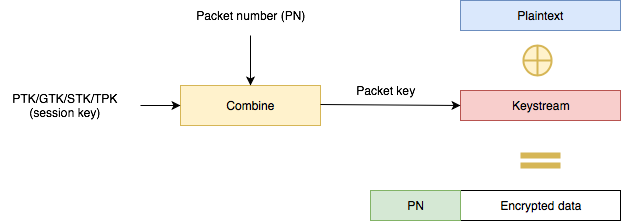
\includegraphics[scale=0.6]{img/SimplifiedEncryption.png}
  \caption[Simplified data encryption]{Simplified data encryption by data confidentiality and integrity protocol.}
  \label{fig:encryption}
\end{figure}

In the diagram, we can see the session key\footnote{Actually, it is only its subkey called transient key (TK), but this detail is not crucial for understanding of the attack principle and could be just confusing fact for the reader.} is mixed with the packet number to establish a packet key. The keystream obtained depends only on the session key and the packet key. Then, keystream is XORed with the plaintext data of the data frame. Finally, we prepend the used packet number to the final packet, to let the receiver decrypt data.

Different packet numbers are used to ensure distinct ciphertexts are produced even when the same plaintext is encrypted multiple times independently with the same key. It is why Vanhoef calls this value nonce because this is precisely its role\footnote{According to Merriem-Webster dictionary~\cite{culpepper_2000merriam}, a nonce is "value occurring, used, or made only once or for a special occasion".}. We can see in Figure~\ref{fig:encryption}, that the encrypted data depend only on these three variables --- session key, packet number, and plaintext data of the frame sent. Hence, when the victim reinstalls an already-in-use session key and resets the packet number, the same combination will be used twice. It is also explicitly stated in the standard revision from 2016~\cite{revision2016} that packet number re-usage breaks the security assumptions of the data confidentiality and integrity protocols. 

The victim also resets the replay counter. As mentioned in the~\ref{sec:security}, this value serves as a protection against replayed frames. Its resetting allows the attacker later replay frames towards the victim.

\subsection{Found Vulnerability} 

The aim of the attacker as described in Section~\ref{subsub:aimOfTheAttacker} is achieved by manipulating and replaying cryptographic handshake messages. The reason why it is possible is because of a vulnerability found in the handshake definition in the standard itself. We are going to show the vulnerability on the 4-way handshake. This attack is targeted against the client. The vulnerability of this handshake is that, when the supplicant receives retransmitted \textit{message~3}, it reinstalls the key already installed, thus, resets the packet number and the replay counter. We will show it in more detail after introducing the state machine of the supplicant as it is defined in the standard.

\begin{figure}[h!]
  \centering
  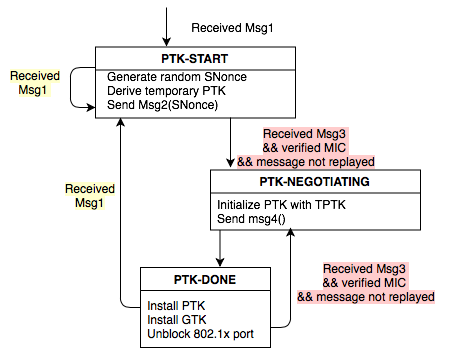
\includegraphics[scale=0.7]{img/SimplifiedStateMachineOfTheHandshake.png}
  \caption[Simplified supplicant state machine of the 4-way handshake]{Simplified supplicant state implementation machine of the 4-way handshake.}
  \label{fig:stateMachineSupplicant}
\end{figure}

A simplified state machine describing how the client (the supplicant) must implement the 4-way handshake is shown in Figure~\ref{fig:stateMachineSupplicant} --- the supplicant transitions to the PTK-START stage when receives \textit{message~1}, either when it is connected to the network for the first time, or when the session key is being refreshed. In this state, the supplicant assembles \textit{message~2} and sends it. The authenticator will reply with \textit{message~3}, which is accepted by the supplicant if the MIC and replay counter is valid. In this case, the supplicant moves to the PTK-NEGOTIATING state, initializes the PTK variable with the temporary PTK variable, sends \textit{message~4} to the authenticator, and transitions to the PTK-DONE state. Now, the PTK and GTK are installed for usage by the data-confidentiality protocol; it unblocks the 802.1x port and thus, the client can send and receive encrypted data frames.~\cite{revision2016}

In Section~\ref{fig:stateMachineSupplicant}, we explicitly highlighted how the supplicant handles retransmitted \textit{messages~1} (yellow) and \textit{3} (red). The attacker uses the fact that the client accepts the \textit{message~3} even if the key is already installed (PTK-DONE), gets back to PTK-NEGOTIATING state and immediately back to PTK-DONE state, where the supplicant installs the PTK and the GTK once again. Thus, reset the packet number and the replay counter. We can also see that if the supplicant gets \textit{message~1} when in PTK-DONE, it goes back to the PTK-START. This can also be used against the client as we will see when monitoring the traffic of the attack in Section~\ref{sec:detectionSystem}.

\subsection{Execution}

We have already explained what the aim is and what is the exploited vulnerability, now we are going to describe how to achieve it. In an infrequent occasion, the vulnerability can be exploited, meaning the packet number can be reused with the same session key, by standard traffic in the Wi-Fi network. This situation can happen due to interference. In Figure~\ref{fig:attackWithoutAttacker}, we show this hypothetical situation.

\begin{figure}[h!]
  \centering
  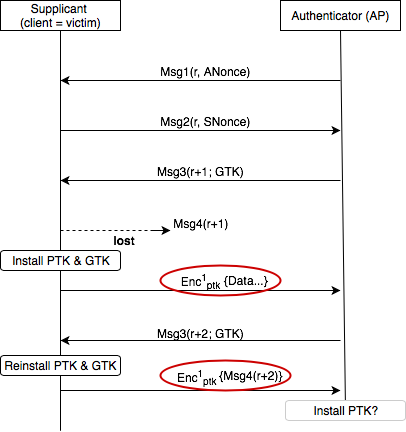
\includegraphics[scale=0.7]{img/attackWithoutAttacker.png}
  \caption[KRACK attack vulnerability exploited because of interference]{KRACK attack vulnerability exploited because of interference without an attacker being present. We assume the victim still accepts the plaintext \textit{message~3} after the PTK is installed; messages using the same packet number are circled red.}
  \label{fig:attackWithoutAttacker}
\end{figure}

First, the authenticator sends \textit{message~1} to the client with replay counter $r$ and randomly generated value ANonce. The supplicant replies to the message by sending \textit{message~2} with the same replay counter $r$ and randomly generated value SNonce. Now, the authenticator derives the PTK as described in Section~\ref{sub:fourWayHandshake} and sends \textit{message~3} with incremented replay counter $r+1$ and GTK encapsulated in Key data field. In response to \textit{message~3}, the supplicant sends \textit{message~4} with the corresponding replay counter $r+1$. The supplicant considers the handshake as completed, installs both the PTK and GTK and in context of the state machine in Figure~\ref{fig:stateMachineSupplicant}, the victim transitions to PTK-DONE state. Unfortunately, the message is lost due to interference. The client starts sending data towards the AP in belief that the handshake was successfully finished. The client uses the packet number of value 1. But the authenticator still did not get the \textit{message~4} of the 4-way handshake. Thus, he thinks that one of the messages \textit{3} or \textit{4} was lost. Therefore, he re-sends the \textit{message~3}. Note, he used incremented replay counter $r+2$. Its incrementation is important. Otherwise, the victim would not accept the message, because it could have been sent by anyone sitting in the middle and monitoring and replaying the traffic. This replay counter is added by a WNIC driver.

Now, we describe how the attacker can trigger the reinstallation. For accomplishing this, the attacker has to, in some cases, establish a channel based Man-in-the-Middle (MitM) position. This attack was found by the same author as the KRACK attacks, in 2014~\cite{Vanhoef:2014}. It is a low-layer attack which allows the adversary to intercept and manipulate the traffic reliably. It solves several problems with establishing a MitM in a Wi-Fi network. Creating a MitM position in a Wi-Fi network is difficult because of the 4-way handshake which negotiates the session key depending on the MAC address of both the AP and the client. Hence, if we use a rogue AP with a different MAC address, the handshake will fail. If we use the real address, the AP and the client would directly communicate with each other. The attack solves these problems by cloning the real AP to a different channel. To perform the attack, we need two Wi-Fi network cards, at least one external. One of them communicates on the channel of the real AP, the other cloning the AP on a different channel. For the implementation of this attack, it is necessary to patch firmware of the wireless network interface card used as a rogue AP. After establishing this position, the attacker can capture, manipulate and block traffic between the client and the real AP. It does not let the adversary decrypt any captured data. Besides other things that had to be patched in the driver, to implement this attack, it was necessary not to let the rogue AP increment the replay counter when sending messages~\cite{Vanhoef:2014}. This is important for the implementation of the KRACK attacks.

When we established the channel based MitM position, we can manipulate and block the data transmitted between the AP and the victim (client). We again assume a client that accepts plaintext retransmissions of \textit{message~3} in the 4-way handshake, when a PTK is already installed. In Figure~\ref{fig:4wayAttackWithDecryption}, we can see several changes. There is now the MitM obtained, the communication with the client on the left is transmitted on a different channel than the communication on the right between the attacker and the real AP. Again, there is shown the 4-way handshake. The principle is the same as in the previous example where no attacker was present except the fact that now the communication goes through the MitM. The MitM only captures and forwards the first three messages and stores these messages to be able to use them later in the communication.

When \textit{message~4} comes from the client, the adversary blocks it, meaning she does not send it further to the real AP. The victim again thinks the 4-way handshake was successfully finished and starts transmitting data. Notice, the victim uses packet number 1 after installation of the PTK and GTK. The AP did not get the acknowledgment in the form of \textit{message~4}. Thus, it re-sends the \textit{message~3} with incremented replay counter towards the MitM, and it forwards it towards the victim. Because the PTK has been installed, the victim answers with the encrypted \textit{message~4} in response and reinstalls the PTK (according to the state machine in Figure~\ref{fig:stateMachineSupplicant}). Next data the victim will send are going to have again the packet number 1. 

Additionally, in this particular case, it is easy to decrypt the data because we captured similar (not the same) encrypted and plaintext messages. A possible way of decrypting these data is shown in Figure~\ref{fig:4wayAttackWithDecryption}. We can see, that in case a message that reuses keystream has known content, it becomes trivial to derive the used keystream. When there is no known content, it is harder to decrypt packets. To do it, we can try to identify packets with known content, for example by their usual length (e.g., DHCP packets). 

\begin{figure}[h!]
  \centering
  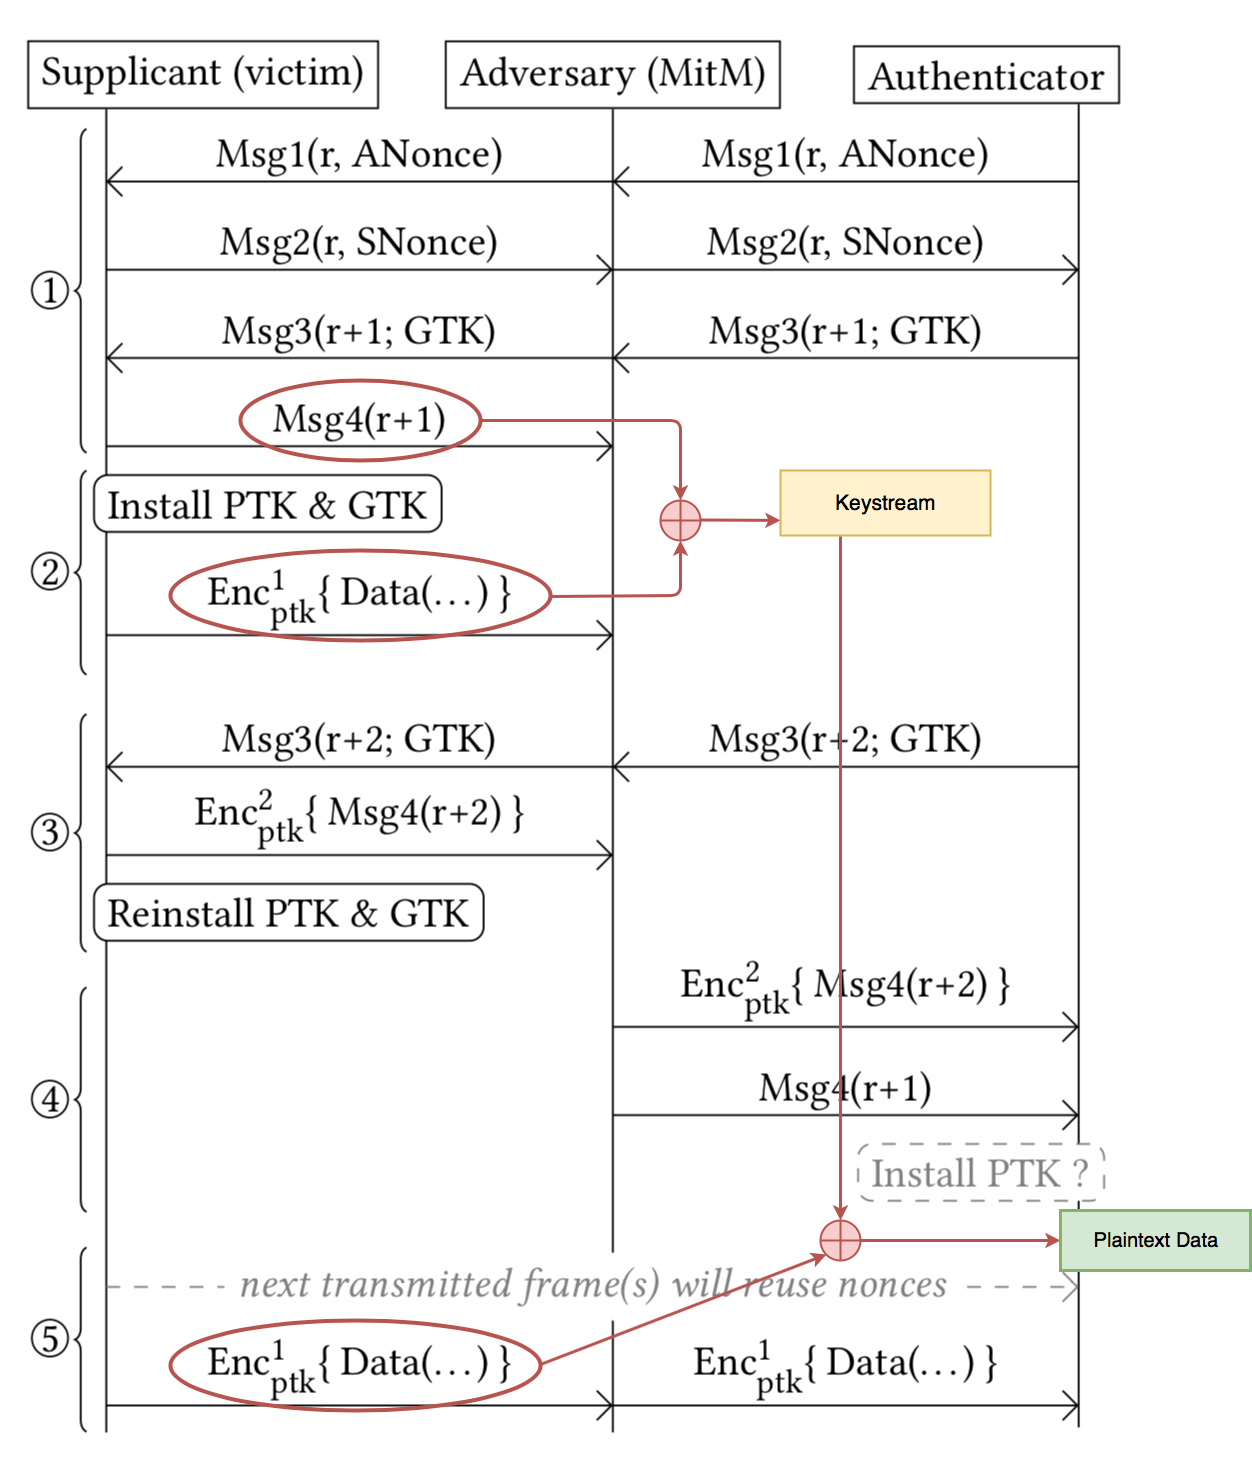
\includegraphics[scale=0.25]{img/xor4wayHandshake.png}
  \caption[KRACK Attack against the 4-way handshake with possible data decryption]{Key reinstallation attack against the 4-way handshake, when the supplicant (victim) still accepts plaintext retransmissions of message 3 if a PTK is installed, possible decryption of data is designated.}
  \label{fig:4wayAttackWithDecryption}
\end{figure}

\subsection{Another variants}

There is also a different variant of the attack against the 4-way handshake. The option depends on the acceptance of the \textit{message~3} by the client. Specifically, it depends if the client accepts the plaintext \textit{message~3} or only encrypted one after installation of the PTK. The process stays the same, but for the implementation, it is necessary to encrypt some captured frames. These specific variants depend on the firmware implementation of the victim. Vanhoef provides a very detailed explanation of different variants of the attack dependent on the handshake attacked and on the implementation of the firmware~\cite{VA_ccs2017, VA_ccs2018}. 

The attack can be targeted either to the AP, in case it is against the the Fast BSS Transition handshake, or the client. 

The attack on each specific handshake is a bit different, but the principle remains the same. The attacker always wants to trick the victim into reinstalling the negotiated or distributed (in case of group key handshake) session key. This can be done by manipulating messages. In some cases, it is necessary to establish the channel based MitM position. When handshake messages do not contain the replay counter, this position is not needed. This situation arises when attacking the Fast BSS Transition and the Fast Initial Link Setup handshake where Authentication and (Re)Association frames are used. Assuming we have the position established (if necessary). Now, we need to monitor data on the channel (or channels, in case of MitM) and store messages that can help us trick the victim to reinstall the session key later in the communication. For this purpose, we primarily need the message that triggers the installation on the side of the victim. In case of the 4-way or PeerKey handshakes, it is \textit{message~3}. In case of the group key handshake, it is \textit{message~1}. \textit{Message~4} or \textit{Message~2} respectively, from the client to the AP then has to be blocked to trick the AP to send another \textit{message~3} or \textit{message~1} respectively, with an incremented replay counter. In case of the Fast BSS Transition handshake, it is the Reassociation Request that we need to store for later re-sending towards the victim. It is similar for remaining vulnerable handshakes. We also have to store the message with reset packet number to be able to decrypt other messages with the same PN used.

\section{Practical impact}

In the time of publication of the exploits, there was a huge number of vulnerable devices. This was because the vulnerability was discovered in the standard itself. The highest impact regarding the number of devices had the 4-way handshake since it is used to mutually authenticate a client and an AP in both WPA and WPA2 protocols. The vulnerability was either in APs or clients. Fortunately, the AP is affected only if supports the standard 802.11r which was released quite recently in 2016. Besides, both personal and enterprise networks were affected. The list of affected vendors is available in~\cite{carnegie_mellon_university_2017} and a community maintained list of available patches in~\cite{kristate_2018}. 

It is also convenient to point out what the attack does not do (by itself). The attack never reveals the WPA pre-shared key or does not compromise corporate credentials via EAP. Besides, when a proper method of encrypted communication is used on a higher layer (VPN, HTTPS, SSH, etc.), it cannot decrypt these data. We assume these services are properly configured. However, Vanhoef~\cite{VA17} warns that this additional layer of protection can be bypassed in non-browser software: in Apple's iOS and OS~X~\cite{langley_2014}, Android~\cite{goodin_2015, Onwuzurike:2015:DMM:2766498.2766522} and VPN~\cite{goodin_2017}. Some of the links provided by the author about this topic were unavailable or out-dated, which may cause some doubt to the reader. Nevertheless, the attack can be used as a base layer for another attack. For example, by decrypting TCP SYN packet, the TCP connection can be hijacked, and malware can be injected into the unencrypted HTTP connections~\cite{VA17}.  

The specific impact of the key reinstallation depends on the attacked data confidentiality and integrity protocol, handshake, and a specific implementation on the side of the victim~\cite{VA_ccs2017}.

\subsection{Attacked Data Confidentiality Protocol}
All three used data confidentiality protocols (TKIP, CCMP, and GCMP) are affected by possible reuse of the keystream which can lead to decryption of the packets. Also, they are vulnerable to replay attacks. The principle of how this is achieved is described in Section~\ref{sec:attackPrinciple}. The possibility of forging frames is given by the attacked encryption algorithm.
When TKIP is used, and we decrypt the packet, we are also able to recover the MIC by attacking the weak Michael algorithm used to authenticate TKIP data frames. When we get the plaintext frame and its encrypted MIC value, we can recover the MIC key~\cite{MichaelIsWeak}. Different MIC is used in each communication direction. Thus, the direction in which we can forge frames depends on the attacked handshake~\cite{VA_ccs2017}.
When CCMP is used, it is only possible to decrypt and replay frames. There are only theoretical attacks that cannot lead to forging packets when reusing the nonce~\cite{ccmpTheoreticalAttacks}.
When GCMP is used, besides decryption and replay, we can forge frames in both directions. It is possible because we can recover the authentication key which is used in both directions~\cite{GCMFailure}.

\subsection{Attacked Handshake}

The direction in which packets can be decrypted (and possibly forged) depends on the handshake being attacked. When the 4-way handshake is attacked (and so, the client), it is possible to decrypt and forge frames sent by the client to the AP. Also, it is possible to replay group addressed frames towards the victim. However, when we attack the AP by attacking the FT handshake, we can decrypt, replay or/and forge frames in the opposite direction.~\cite{VA_ccs2017}

\subsection{Specific Implementation}

The most vulnerable devices where using wpa\_supplicant of version 2.4 and above. This issue is further described in the original research~\cite{VA_ccs2017}. This open source software implementation of the supplicant is used on Linux and Android 6.0 and above. It turned out this implementation could be tricked into reinstalling an all-zero key, allowing full decryption of all data sent by the client.

Also, it was found that the implementation of iOS and Windows operating systems did not properly follow the standard and thus, they were not vulnerable to PTK reinstallation.

In different implementation specifics, there were no such differences, and all the small nuances are precisely described in the original research~\cite{VA_ccs2017, VA_ccs2018}.

\section{Countermeasures}
\label{sec:countermeasures}
We can look at the countermeasures necessary to be taken from two perspectives. The first is from the affected user --- the other one then from the developer. 

\subsection{User Point of View}
To be protected against the attack, it is necessary to update affected devices. There are lists of available patches to check if the specific device has been patched or not~\cite{kristate_2018}. As it has been said, an AP is vulnerable only if it supports standard 802.11r. Otherwise, it does not have to be updated. To be protected against all other KRACK attacks, it is necessary to patch the vulnerable client. The AP can be patched to protect a client side too. But if the client connects to another network and the AP does not also have the setting to protect clients, the client is still vulnerable. This protection on the side of the AP is based on the prohibition of the retransmission of message 3 of the 4-way handshake. One of the APs running with this protection setting available is with operating system OpenWrt. However, this setting can lead to worse performance of the network, especially in case of a place with high interference.

\subsection{Developer Point of View}

From the developer point of view, the main countermeasure that should take place is to prevent reinstallation of the key that was already used with the same session key or is in use right now. 
Vanhoef proposes two mitigation techniques. The first should be taken by the entity implementing the data-confidentiality protocol. This entity should check whether an already-in-use key is being installed and in such a case, take care that associated nonces and replay counters are not reset. In this case, it is necessary to increase the replay counter of received group key handshake messages. Otherwise, an adversary can use an old group \textit{message~1} to make a victim temporarily install an old (different) key, to subsequently reinstall the current group key using a more recent group \textit{message~1}.~\cite{VA_ccs2017}
A second proposed solution is to add a boolean variable to the state machine illustrated in Figure~\ref{fig:stateMachineSupplicant}. This variable would be initialized to false and set to true when a new PTK in PTK-START state is generated. If the supplicant is entering the PTK-DONE and the variable is true, the PTK is installed, and the boolean is set back to false. Otherwise, the installation of the PTK is skipped.~\cite{VA_ccs2017} 
The author also notified vendors about the vulnerability and helped to develop or design some implemented countermeasures~\cite{VA17}. 
 

 
